\section{Quadratische Funktionen}
\subsection{Einführungsaufgabe}
Alice wirft einen Ball mit einer Geschwindigkeit von $8$ m/s senkrecht nach oben.
In der Nähe der Erdoberfläche kann die Höhe des Balls $t$ Sekunden nach dem Abwurf durch die folgende Funktion beschrieben werden:
\[h(t)=-5t^2+8t+1.5\]
\begin{enumerate}
    \item 	Überlegen Sie, ohne zu rechnen: Wie erwarten Sie, wird der Graph von $h$ ungefähr aussehen?
    \item 	Zeichnen Sie den Graphen von $h$. Sie können dazu auch www.geogebra.org benutzen. Dazu müssen Sie ins Eingabefeld
          \lstset{basicstyle=\ttfamily}
          \begin{lstlisting}
            h(x) = -5*x^2 + 8*x + 1.5
            \end{lstlisting}
          tippen.
          Übertragen Sie den Graphen in das Koordinatensystem unten:
          \begin{center}
              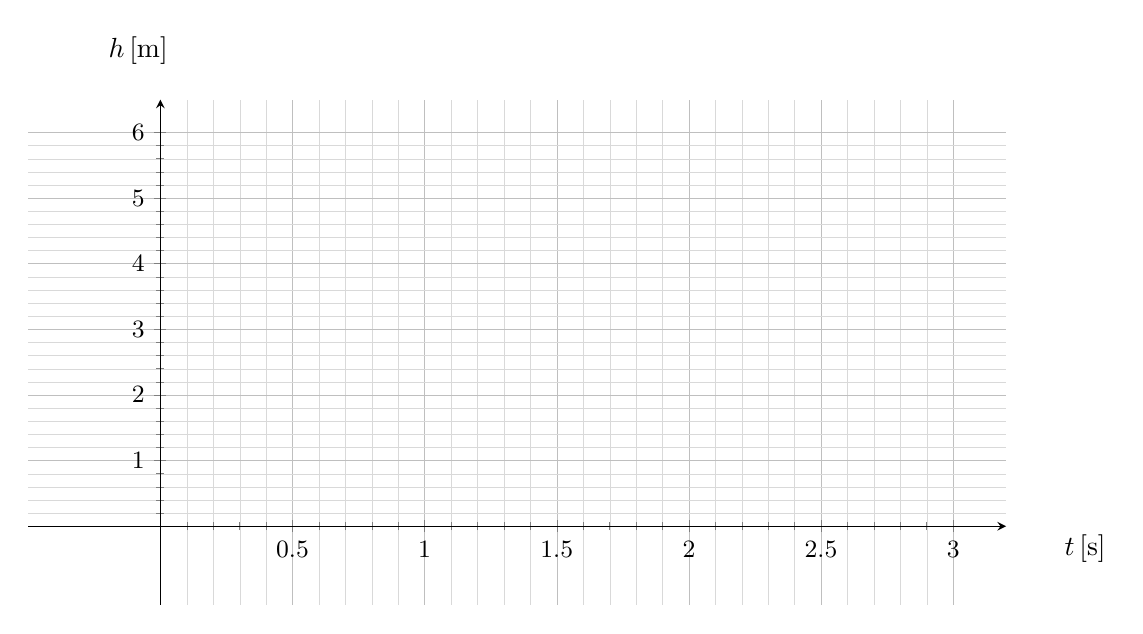
\begin{tikzpicture}
                  \begin{axis}[
                          axis lines=middle,
                          xmin=-0.5, xmax=3.2,
                          ymin=-1.2, ymax=6.5,
                          xtick={0,0.5,1,1.5,2,2.5,3},
                          ytick={0,1,2,3,4,5,6},
                          minor x tick num=4,
                          minor y tick num=4,
                          xlabel={$t\,[\mathrm{s}]$},
                          ylabel={$h\,[\mathrm{m}]$},
                          xlabel style={below right},
                          ylabel style={above left},
                          enlargelimits=false,
                          grid=both,
                          major grid style={line width=0.2pt, draw=gray!50},
                          minor grid style={line width=0.1pt, draw=gray!30},
                          tick label style={font=\small},
                          every axis x label/.style={at={(ticklabel* cs:1.05)},anchor=west},
                          every axis y label/.style={at={(ticklabel* cs:1.05)},anchor=south},
                          x label style={yshift=-8pt},
                          y label style={xshift=-8pt},
                          width=14cm,
                          height=8cm
                      ]

                      % Optional: Beispielkurve
                      %\addplot[domain=0:3, thick, blue] {6 - 4.9*x^2};

                  \end{axis}
              \end{tikzpicture}
          \end{center}
    \item Welche Punkte des Graphen sind besonders interessant? Welche Bedeutung haben die Koordinaten dieser Punkte im Kontext des Ballwurfes?
    \item Beschreiben Sie den Graphen mithilfe der Fachbegriffe \textbf{Nullstellen}, \textbf{y-Achsenabschnitt}, \textbf{Monotonie}, \textbf{Symmetrie (gerade, ungerade)}
\end{enumerate}
\newpage

\subsection{Einführung, Definition, Normalparabel}
Nachdem wir die linearen Funktionen genauer untersucht haben, widmen wir uns nun dem Studium einer neuen Klasse von Funktionen: Die sogenannte quadratische Funktion.
\begin{deff}[Quadratische Funktion]{}
    Eine Funktion der Form
    \[f(x)=ax^2+bx+c\]
    mit $a\neq 0$ heisst quadratische Funktion.
    Der Graph einer solchen Funktion heisst Parabel.
\end{deff}
\begin{examplebox}{}
    Die Funktion aus der Einführungsaufgabe
    \[h(t)=-5t^2+8t+1.5\]
    ist eine quadratische Funktion mit den Koeffizienten $a=-5,\ b=8$ und $c=1.5$.
\end{examplebox}
Eine besondere Stellung unter den quadratischen Funktionen hat die sogenannte Quadratfunktion und deren Graphen inne:

\begin{deff}[]{}
    Ein Spezialfall der quadratischen Funktionen ist die Quadratfunktion $f(x)=x^2$. Der Graph dieser Funktion heisst \textbf{Normalparabel}.
    \begin{center}
        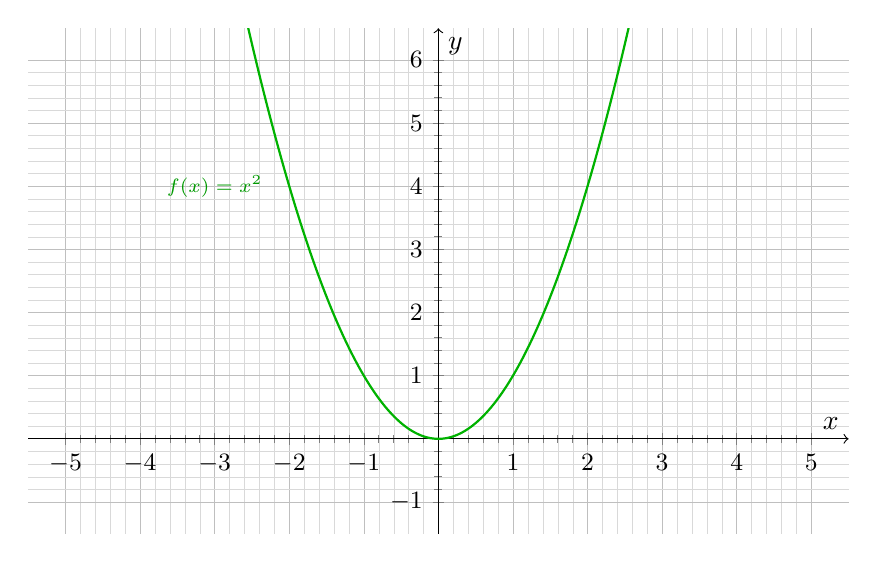
\begin{tikzpicture}
            \begin{axis}[
                    axis lines=middle,
                    xlabel={$x$},
                    ylabel={$y$},
                    xmin=-5.5, xmax=5.5,
                    ymin=-1.5, ymax=6.5,
                    xtick={-5,-4,...,5},
                    ytick={-1,0,...,6},
                    minor x tick num=4,
                    minor y tick num=4,
                    grid=both,
                    major grid style={line width=0.2pt, draw=gray!50},
                    minor grid style={line width=0.1pt, draw=gray!30},
                    tick label style={font=\small},
                    enlargelimits=false,
                    axis line style={->},
                    width=12cm,
                    height=8cm,
                    samples=200
                ]

                % Funktion f(x) = x^2
                \addplot[
                    domain=-3:3,
                    thick,
                    green!70!black
                ] {x^2};

                % Funktionsbeschriftung
                \node at (axis cs:-3,4) {\scriptsize\textcolor{green!60!black}{$f(x) = x^2$}};

            \end{axis}
        \end{tikzpicture}
    \end{center}
\end{deff}
Einige Eigenschaften der Normalparabel:
\begin{itemize}
    \item Alle Punkte befinden sich auf oder über der x-Achse. Anders gesagt: Die Wertemenge der Quadratfunktion ist $\mathbb{R}^+_0$. Dies ist so, weil das Quadrat einer reellen Zahl stets nicht negativ ist.
    \item Sie verläuft achsensymmetrisch zur y-Achse. Anders gesagt: Die Quadratfunktion ist gerade. Dies lässt sich leicht prüfen:
          \begin{align*}
              f(-x)=(-x)^2 = x^2 =f(x)
          \end{align*}
    \item Sie besitzt bei $(0,0)$ einen tiefsten Punkt, denn $f(0)=0^2=0$ und für alle $x\neq 0$ gilt $f(x)>0$.
\end{itemize}
Solche oder ähnliche Eigenschaften haben auch die anderen quadratischen Funktionen. Mehr dazu im nächsten Teilkapitel...
% \subsubsection{Polynomfunktionen}
% Die quadratischen Funktionen gehören wie auch die linearen Funktionen zur Klasse der Poly-nomfunktionen. Eine Vielzahl von Zusammenhängen, die in Naturwissenschaften, Technik, Wirt-schaft und natürlich in der Mathematik untersucht werden gehören zu diesem Typ Funktionen. Beispiele für Polynomfunktionen sind:
% \begin{align*}
%      & f(x) = 2x+3                          &  & f(x)=3x^2-18 \\
%      & f(x) = 23x^{12}-4x^{11}+23x^7+2x^4-1 &  & f(x)=x^4+x^2
% \end{align*}
% \begin{itemize}
%     \item Den grössten Exponenten von $x$ nennt man den \textbf{Grad} der Funktion. Im Beispiel oben haben wir eine (Polynom-) Funktion 1. Grades, eine 2. Grades, eine 12. Grades und eine 4. Grades.
%     \item Die Funktionen ersten Grades kennen wir schon. Man nennt sie auch lineare Funktionen.
%     \item Auch die Gleichung 2. Grades haben wir gerade kennengelernt: es sind die quadratischen Funktionen.
% \end{itemize}
% \begin{deff}[Polynomfunktion]{}
%     Sei $n\in\mathbb{N}$. Eine Funktion heisst \textbf{Polynomfunktion n-ten Grades}, wenn ihre Gleichung die folgende Form hat:
%     \[f(x)=a_n x^n+a_{n-1} x^{n-1}+\cdots+a_1 x+a_0,\]
%     Wobei $a_n,\ a_{n-1},\dots, a_0$ allesamt feste reelle Zahlen sind (Koeffizienten genannt) und $a_n\neq 0$ ist
% \end{deff}
% \subsubsection{Übungen}
% \begin{enumerate}
%     \item 	Welche der folgenden Funktionen sind Polynomfunktionen? Geben Sie auch den Grad an.
%           \begin{enumerate}
%               \item $y=-7x^5+12x^2-14$
%               \item $y=(x^3+3)^2$
%               \item $y=x+1+x^{-1}$
%               \item $y=\sqrt{3}\cdot x^2+2$
%               \item $y=(x+1)^3-x^3-3x^2$
%               \item $y=2\sqrt{x}$
%               \item $y=2^x-1024$
%           \end{enumerate}
%     \item Welche der folgenden Funktionen sind quadratische Funktionen?
%           Geben Sie die Koeffizienten $a,b$ und $c$ an.
%           \begin{enumerate}
%               \item $y=12-3x+2x^2$
%               \item $y=x^2-4$
%               \item $y=2(x-3)^2+3$
%               \item $y=(2x-1)^3$
%               \item $y=\frac{1}{x^2+3x+4}$
%               \item $y=(x+2)^3-x(x-1)^2$
%           \end{enumerate}
% \end{enumerate}
% \subsubsection{Lösungen}
% \begin{enumerate}
%     \item 	Welche der folgenden Funktionen sind Polynomfunktionen? Geben Sie auch den Grad an.
%           \begin{enumerate}
%               \item Polynomfunktion 5. Grades
%               \item Polynomfunktion 6. Grades
%               \item Keine Polynomfunktion
%               \item Polynomfunktion 2. Grades
%               \item Polynomfunktion 1. Grades
%               \item Keine Polynomfunktion
%               \item Keine Polynomfunktion
%           \end{enumerate}
%     \item Welche der folgenden Funktionen sind quadratische Funktionen? Geben Sie die Koeffizienten $a,b$ und $c$ an.
%           \begin{enumerate}
%               \item $a=2,b=-3,c=12$
%               \item $a=1,b=0,c=-4$
%               \item $a=2,b=-12,c=21$
%               \item Nicht quadratisch
%               \item Nicht quadratisch
%               \item $a=8,b=11,c=8$
%           \end{enumerate}
% \end{enumerate}
\newpage
\subsection{Der Graph quadratischer Funktionen}
Wir wissen bereits wie der Graph der quadratischen Funktion $y=x^2$ aussieht. Die Normalparabel hat folgende Eigenschaften:
\begin{itemize}
    \item sie ist symmetrisch bezüglich der y-Achse
    \item sie hat im Ursprung den tiefsten Punkt - den sogenannten \textbf{Scheitel}
\end{itemize}
Bei der Normalparabel ist $a=1,\ b=c=0$.

%Wir untersuchen nun den Einfluss die die drei Koeffizienten $a,\ b$ und $c$ auf die Gestalt des Graphen haben.
In diesem Kapitel soll untersucht werden, inwiefern sich die Graphen der anderen quadratischen Funktionen von der Normalparabel unterscheiden, was die Gemeinsamkeiten sind und welchen Einfluss die drei Koeffizienten a,b und c auf die Gestalt des Graphen haben.
\subsubsection{Einführungsaufgabe}
Verwenden Sie die Geogebra-App, um die folgenden Fragen zu beantworten:
\begin{enumerate}
    \item Geogebra-Vorbereitung:
          \begin{enumerate}
              \item Tippen Sie $y=x^2$ ins Eingabefenster, damit die Normalparabel angezeigt wird. Sie dient und als Vergleich.
              \item Tippen Sie nun $y=ax^2+bx+c$ ins Eingabefenster. Damit werden drei Schieberegler erzeugt und der Graph der Funktion wird angezeigt. Mit den Schiebereglern lassen sich die Werte der Koeffizienten verändern und die Kurve passt sich entsprechend an.
          \end{enumerate}
          Für den Fall, dass mit Geogebra etwas schiefläuft, finden Sie das Ganze auch als Applet auf Moodle.
    \item Setzten Sie die Koeffizienten $a$ auf $1$ und $b$ auf $0$. Variieren Sie nun den Koeffizienten $c$. Wie verändert sich der Graph der Funktion? Versuchen Sie, eine Erklärung dafür zu formulieren.
    \item Setzten Sie die Koeffizienten $b$ auf $0$ und $c=0$. Variieren Sie nun den Koeffizienten $a$. Wie verändert sich der Graph der Funktion? Wann ist die Parabel nach unten geöffnet? Versuchen Sie wieder, eine Erklärung dafür zu formulieren.

          Was passiert, wenn $a\neq 1$ ist und Sie $c$ verändern?
    \item Setzten Sie nun die Koeffizienten $a$ auf $1$ und $c=0$. Variieren Sie nun den Koeffizienten $b$. Was geschieht mit der Parabel?
\end{enumerate}
\newpage
\subsubsection{Erste Beobachtungen und Vermutungen}
Lesen Sie diesen Text aus dem MINT-Lernzentrum der ETH Zürich:
\bigskip

{\it
    Was haben wir bisher verstanden? Dass die Normalparabel eine nach oben offene, gekrümmte und bezüglich der y-Achse symmetrische Kurve mit dem Ursprung als tiefstem Punkt sein muss, ist leicht nachvollziehbar. Und die Lernaufgabe hat sicherlich dazu beigetragen, dass wir genauer durchschauen, wie sich (verglichen mit der Normalparabel) der Graph verändert, wenn wir statt $a=1$ einen anderen Koeffizienten $a$ wählen und/oder wenn wir statt $c=0$ eine andere additive Konstante $c$ wählen.
    \medskip

    Wählt man statt $f:y=x^2$  die Funktion $y=ax^2$, so wird jeder einzelne Funktionswert von $f$ mit derselben Konstanten a multipliziert. Ist $a>1$, so wird also jeder einzelne Funktionswert um diesen Faktor vergrössert; ist aber $0<a<1$, so wird jeder einzelne Funktionswert um diesen Faktor verkleinert. Negative $a$-Werte schliesslich \glqq klappen\grqq{} die Parabel nach unten. Man kann also auch sagen: Der Koeffizient $a$ beeinflusst die \glqq Öffnungsweite\grqq{} der Parabel und bestimmt zudem, ob diese nach oben oder nach unten geöffnet ist.
}

\begin{center}
    \begin{tikzpicture}
        \begin{axis}[
                axis lines=middle,
                xmin=-5, xmax=5,
                ymin=-8, ymax=25,
                xtick={-4,-3,...,4},
                ytick={0,5,10,15,20},
                xlabel={$x$},
                ylabel={},
                enlargelimits=true,
                axis line style={->},
                tick style={draw=none},
                clip=false,
                width=12cm, height=10cm,
                samples=100
            ]

            % Originalparabel x^2
            \addplot [domain=-4.5:4.5, thick] {x^2};
            \node at (axis cs:-3.5,15) {$x^2$};

            % a > 1
            \addplot [domain=-3.5:3.5, dashed] {2*x^2};
            \node at (axis cs:-2.5,23) {$a > 1$};

            % 0 < a < 1
            \addplot [domain=-4.5:4.5, dashed] {0.5*x^2};
            \node at (axis cs:-4.7,5.5) {$0 < a < 1$};

            % a < 0
            \addplot [domain=-3.5:3.5, dashed] {-0.5*x^2};
            \node at (axis cs:-3,-6.5) {$a < 0$};

            % Punkt (3,9) und gestrichelte Linien
            %\draw[dashed] (axis cs:3,0) -- (axis cs:3,9);
            %\draw[dashed] (axis cs:0,9) -- (axis cs:3,9);
            %\node at (axis cs:3,-0.5) {$3$};
            %\node at (axis cs:-0.5,9) {$9$};

            % Punkt auf x^2 bei x=3
            %\fill (axis cs:3,9) circle[radius=2pt];

        \end{axis}
    \end{tikzpicture}
\end{center}
{\it
Ebenso klar ist, welchen graphischen Effekt das Addieren einer Konstanten $c$ zu $y=x^2$  bewirkt. Wie von einem unsichtbaren Lift bewegt, wird die Normalparabel einfach um die entsprechende Zahl in y-Richtung verschoben, weil jeder einzelne Funktionswert der Funktion $y=x^2$ nun um den Wert $c$ vergrössert (bzw. verkleinert) wird.
}
\begin{center}
    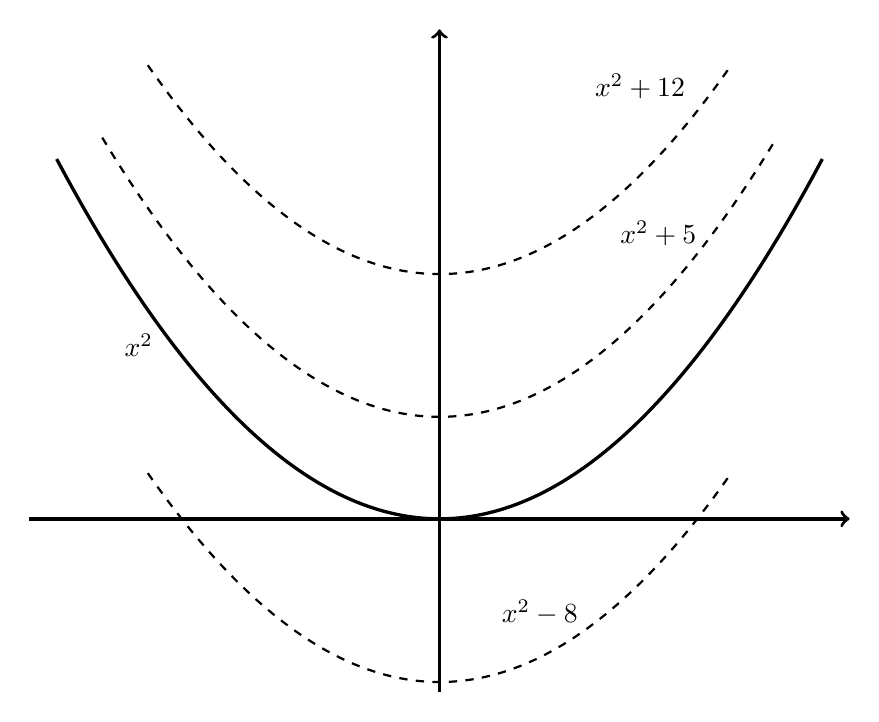
\begin{tikzpicture}
        \begin{axis}[
                axis lines=middle,
                xmin=-4.5, xmax=4.5,
                ymin=-8.5, ymax=24,
                xtick=\empty,
                ytick=\empty,
                axis line style={->, very thick},
                enlargelimits=false,
                clip=false,
                width=12cm, height=10cm,
                samples=200
            ]

            % x^2
            \addplot[domain=-4.2:4.2, very thick] {x^2};
            \node at (axis cs:-3.3,8.5) {$x^2$};

            % x^2 + 5
            \addplot[domain=-3.7:3.7, dashed, thick] {x^2 + 5};
            \node at (axis cs:2.4,14) {$x^2 + 5$};

            % x^2 + 12
            \addplot[domain=-3.2:3.2, dashed, thick] {x^2 + 12};
            \node at (axis cs:2.2,21.2) {$x^2 + 12$};

            % x^2 - 8
            \addplot[domain=-3.2:3.2, dashed, thick] {x^2 - 8};
            \node at (axis cs:1.1,-4.6) {$x^2 - 8$};

        \end{axis}
    \end{tikzpicture}
\end{center}
{\it
Bezüglich des Einflusses des Koeffizienten $b$ hat die Lernaufgabe jedoch noch keine definitive Klarheit gebracht. Die vielleicht naheliegende Vermutung, dass $b$ einfach nur eine horizontale Verschiebung verursacht, hat sich als falsch erwiesen. Daraus erwächst eine gewisse Spannung...
\medskip

Alle bisherigen Untersuchungen nähren aber die Vermutung, dass der Graph einer quadratischen Funktion stets \glqq ähnlich wie die Normalparabel \grqq{} aussieht, nur eventuell verschoben oder in der \glqq Öffnungsweite\grqq{} verändert oder nach unten geöffnet. Genauer: Der Graph ist immer achsensymmetrisch bezüglich der vertikalen Achse durch den tiefsten beziehungsweise höchsten Punkt des Graphen, den man Scheitelpunkt nennt. Noch präziser formulieren wir hier die folgende Vermutung:
}
\medskip

\begin{fazit}[Vermutungen]{}
    \begin{itemize}
        \item Der Graph einer quadratischen Funktion hat stets ein Extremum, den sog. \textbf{Scheitelpunkt}. Es bleibt zu klären, wo dieser Scheitelpunkt genau liegt.
        \item Der Graph ist stets achsensymmetrisch bezüglich der vertikalen Achse durch den Scheitelpunkt.
              Der Graph ist nach oben geöffnet, falls $a>0$ ist und nach unten, falls $a<0$ ist.
        \item Der Graph ist stets \glqq ähnlich\grqq{} zur Normparabel. Eventuell verschoben, gestreckt und/oder gespiegelt.
    \end{itemize}
\end{fazit}
\newpage

\subsubsection{Öffnung und Scheitelpunkt}
Die folgenden Vorüberlegungen bereiten Sie auf die wichtigsten Schritte im Beweis der Vermutungen rund um die Gestalt der Graphen quadratischer Funktionen vor:
\begin{enumerate}
    \item Erklären Sie, wieso der Term $x^2+3$ stets grösser oder gleich $3$ ist, unabhängig davon, welche Zahl man für $x$ einsetzt.
          \kariert{8}

    \item Erklären Sie, wieso der Term $\frac{7}{3} (x-2)^2+6$ stets grösser oder gleich $6$ ist, unabhängig davon, welche Zahl man für $x$ einsetzt.
          \kariert{8}

    \item Erklären Sie, wieso der Term $-3(x+5)^2+9$ stets kleiner oder gleich $9$ ist, unabhängig davon, welche Zahl man für $x$ einsetzt.
          \kariert{8}

    \item 	Welche Zahl muss man im Term aus Aufgabe 2 für $x$ einsetzen, damit der Term den kleinstmöglichen Wert annimmt?
          \kariert{6}
          \newpage
    \item Welche Zahl muss man im Term aus Aufgabe $3$ für $x$ einsetzen, damit der Term den grösstmöglichen Wert annimmt?
          \kariert{8}

    \item Hat der Term $2(3x-14)^2-17$ einen grössten oder einen kleinsten Wert? Welchen Wert ist das und welche Zahl muss man dafür für $x$ einsetzen?
          \kariert{8}

    \item Der Graph einer Funktion $f$ ist genau dann symmetrisch zur y-Achse, wenn für jeden Input $\epsilon \in \mathbb{D}_f$ gilt.

          \[
              f(-\epsilon)=f(\epsilon)
          \]
          Formulieren Sie eine ähnliche Gleichung für eine Funktion $g$, deren Graphen Achsensymmetrisch bezüglich der vertikalen Geraden $x=3$ verläuft.
          \kariert{20}

\end{enumerate}
\newpage

Mit den Vorüberlegungen kann man nun leicht nachvollziehen, dass Graphen von quadratischen Funktionen einen höchsten oder tiefsten Punkt besitzen (Scheitelpunkt) und symmetrisch bezüglich einer Vertikalen durch den Scheitelpunkt verlaufen. Betrachten Sie dazu das Folgende:

\begin{examplebox}{}
    Gegeben ist die Funktion $f(x)=2x^2+12x-22$. Zuerst wird der Funktionsterm in eine \glqq besser deutbare\grqq{} Form umgewandelt. Zu diesem Zweck wird als erstes der Vorfaktor $a=2$ von $x^2$ ausgeklammert:
    \[
        f(x)=2(x^2+6x-11)
    \]
    Wir ergänzen den Term $x^2 + 6x$ quadratisch:
    \begin{align*}
        f(x) & = 2(\underbrace{x^2 +6x + \textcolor{red}{9}}_{=(x+3)^2} - \textcolor{red}{9} - 11) \\
             & = 2((x+3)^2-20)                                                                     \\
        f(x) & =2(x+3)^2-40
    \end{align*}
    Da $2(x+3)^2$ für jedes $x\in \mathbb{R}$ stets nicht negativ ist, und genau dann $0$ ist, wenn $x=-3$ ist, hat der Graph der Funktion $f$ einen tiefsten Punkt in $S=(-3,-40)$.

    Ausserdem verläuft der Graph der Funktion $f$ symmetrisch bezüglich der vertikalen Geraden $x=-3$, denn für alle $\epsilon \in \mathbb{R}$ gilt
    \[f(-3+\epsilon) = 2((-3+\epsilon)+3)^2-40=2\epsilon^2-40\]
    und
    \[f(-3-\epsilon) = 2((-3-\epsilon)+3)^2-40=2(-\epsilon)^2-40 = 2\epsilon^2 -40\]
    Also
    \[f(-3+\epsilon) = f(-3-\epsilon)\]

    \begin{center}
        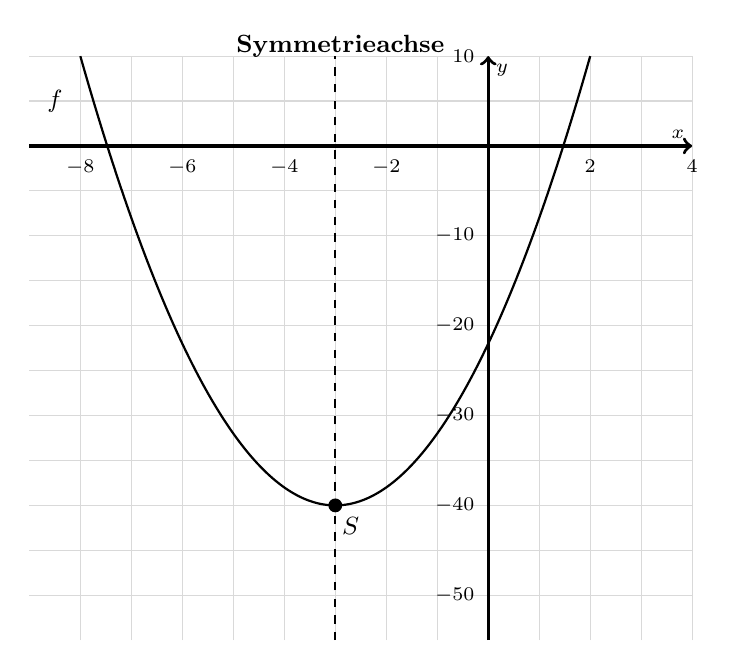
\begin{tikzpicture}
            \begin{scriptsize}
                \begin{axis}[
                        xmin=-9, xmax=4,
                        ymin=-55, ymax=10,
                        axis lines=middle,
                        grid=both,
                        minor tick num=1,
                        axis line style={->, very thick},
                        tick style={draw=none},
                        xlabel={$x$},
                        ylabel={$y$},
                        samples=200,
                        width=10cm, height=9cm,
                        xtick={-8,-6,...,4},
                        ytick={-50,-40,...,10},
                        enlargelimits=false,
                        grid style={gray!30},
                        clip=false
                    ]

                    % Parabel f(x)
                    \addplot[domain=-8:2, thick] {2*x^2 + 12*x - 22};
                    \node at (axis cs:-8.5,5) {\small$f$};

                    % Scheitelpunkt
                    \fill (axis cs:-3,-40) circle (2.5pt);
                    \node at (axis cs:-2.7,-42.3) {\small$S$};

                    % Symmetrieachse gestrichelt
                    \draw[dashed, thick] (axis cs:-3,-55) -- (axis cs:-3,10);
                    \node at (axis cs:-2.9,9) [above] {\small\textbf{Symmetrieachse}};
                \end{axis}
            \end{scriptsize}
        \end{tikzpicture}
    \end{center}
\end{examplebox}
\newpage

Als Beweis für die aufgestellten Vermutungen werden im Folgenden in einem Text des MINT-Lernzentrums der ETH Zürich, die gleichen Umformungsschritte, wie im Beispiel an der allgemeinen quadratischen Funktion durchgeführt:

Bezüglich der oben formulierten Vermutung können wir nun absolute Sicherheit erlangen und gleichzeitig die vagen Punkte präzisieren. Dazu nehmen wir an, es liegt uns eine beliebige quadratische Funktion $f(x)=ax^2+bx+c$ vor.
Wir führen mit dem Funktionsterm eine quadratische Ergänzung durch und erhalten:
\begin{align*}
    f(x) & =ax^2+bx+c                                                                                            \\
         & =a \left(x^2+\frac{b}{a} x+\frac{c}{a}\right)                                                         \\
         & =a \left(x^2+\frac{b}{a} x+\left(\frac{b}{2a}\right)^2-\left(\frac{b}{2a}\right)^2+\frac{c}{a}\right) \\
         & =a\left[\left(x+\frac{b}{2a}\right)^2-\frac{b^2}{4a^2}+\frac{c}{a}\right]                             \\
         & =a\left(x+\frac{b}{2a}\right)^2-\frac{b^2}{4a}+c                                                      \\
         & =a\underbrace{\left(x+\frac{b}{2a}\right)^2}_{V}+\underbrace{c-\frac{b^2}{4a}}_{H}\ \ (*)
\end{align*}
Wir haben den Funktionsterm nun also dargestellt als Summe eines ver-a-fachten vorderen Terms $V$ und eines hinteren Terms $H$. Was können wir über die einzelnen Bestandteile von (*) aussagen? Nun, sicherlich ist $H$ konstant, also unabhängig von $x$, weil die Unbekannte darin gar nicht vorkommt. Und $V$ ist grösser oder gleich $0$, egal, welche Zahl man für $x$ einsetzt. $V$ nimmt also seinen kleinsten Wert (nämlich $0$) an, falls wir für $x$ die Zahl $-\frac{b}{2a}$ einsetzen. Und für jede andere Belegung der Variablen wird $V > 0$ sein und desto grösser, je weiter sich $x$ von diesem Wert entfernt.

Da $a$ eine beliebige reelle Zahl sein darf, empfiehlt sich eine Fallunterscheidung:
\begin{description}
    \item[Fall a > 0:] 	In diesem Fall ist $H$ der kleinstmögliche Wert, den der Term (*) überhaupt annehmen kann, nämlich einzig dann, wenn wir für $x$ die Zahl $-\frac{b}{2a}$ einsetzen. Dann nämlich verschwindet $V$. Die Funktion $f$ hat also ein Minimum: Dem Input $x=-\frac{b}{2a}$ wird der kleinstmögliche Funktionswert $c-\frac{b^2}{4a}$ zugeordnet.
    \item[Fall a < 0:] In diesem Fall ist $H$ der grösstmögliche Wert, den der Term (*) überhaupt annehmen kann, nämlich einzig dann, wenn wir für $x$ die Zahl $-\frac{b}{2a}$ einsetzen. Dann nämlich verschwindet $V$. Die Funktion $f$ hat also ein Maximum: Dem Input $x=-\frac{b}{2a}$ wird der grösstmögliche Funktionswert $c-\frac{b^2}{4a}$ zugeordnet.
\end{description}

Insgesamt haben wir also Folgendes eingesehen:
\medskip

\begin{theo}[Öffnung und Scheitelpunkt quadratischer Funktionen]{}
    Der Graph der quadratischen Funktion $f:x \mapsto ax^2+bx+c$ ist nach oben geöffnet, wenn $a>0$ und nach unten geöffnet, wenn $a<0$.

    Der Graph hat genau ein Extremum: Den Scheitelpunkt $S$ mit den Koordinaten
    \[
        S=(x_s,y_s )=\left(-\frac{b}{2a},c-\frac{b^2}{4a}\right)=\left(-\frac{b}{2a},f\left(-\frac{b}{2a}\right)\right)
    \]
\end{theo}
\subsubsection{Achsensymmetrie}
Wir vermuten ja noch eine Achsensymmetrie des Graphen bezüglich der vertikalen Achse durch den Scheitelpunkt, also bezüglich der Geraden $x=x_s$. Wie können wir diese Symmetrie nachweisen?

Ganz einfach: Wenn wir zwei Inputs wählen, einen links und einen rechts von der Stelle $x=x_s$ auf der x-Achse, aber so, dass sie gleich weit entfernt von der x-Koordinate des Scheitelpunktes sind, dann erwarten wir gleiche Outputs. Wir erwarten also, dass
\[
    f(x_x-\epsilon) = f(x_s+\epsilon)
\]
sein wird für alle $\epsilon \in \mathbb{R}$.

\begin{center}
    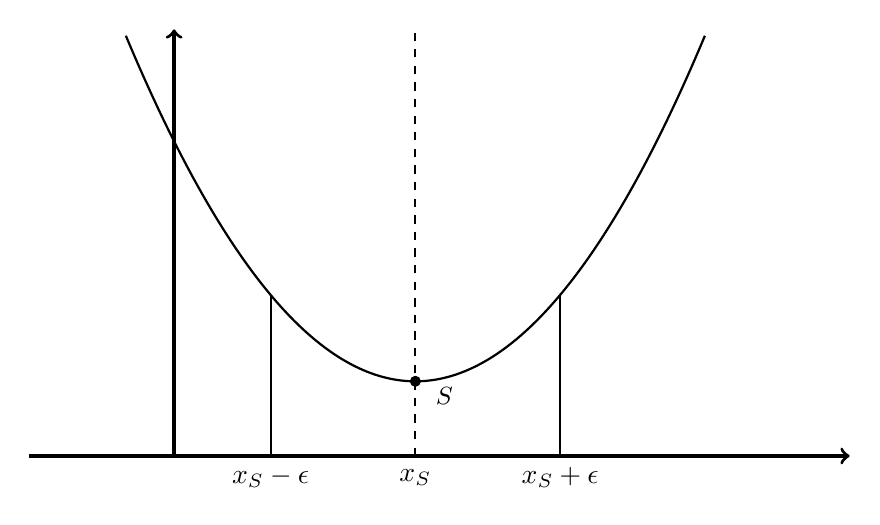
\begin{tikzpicture}
        \begin{axis}[
                xmin=-1.5, xmax=7,
                ymin=0, ymax=20,
                axis lines=middle,
                axis line style={->, very thick},
                tick style={draw=none},
                xtick=\empty,
                ytick=\empty,
                samples=200,
                width=12cm, height=7cm,
                grid=both,
                minor tick num=1,
                grid style={gray!30},
                clip=false,
                xlabel={}, ylabel={}
            ]

            % Parabel f(x) = x^2 + 5, komplett oberhalb der x-Achse
            \addplot[domain=-0.5:5.5, thick] {1.8*(x-2.5)^2 + 3.5};
            %\node at (axis cs:-4.2,7) {\small$f$};

            % Scheitelpunkt
            \fill (axis cs:2.5,3.5) circle (2pt);
            \node at (axis cs:2.8,2.8) {\small$S$};

            % Symmetrieachse
            \draw[dashed, thick] (axis cs:2.5,0) -- (axis cs:2.5,20);
            \node at (2.5, -1) {$x_S$};

            \draw[thick] (axis cs:1,0) -- (axis cs:1,7.55);
            \node at (1, -1) {$x_S-\epsilon$};

            \draw[thick] (axis cs:4,0) -- (axis cs:4,7.55);
            \node at (4, -1) {$x_S+\epsilon$};
        \end{axis}
    \end{tikzpicture}
\end{center}
In der quadratisch ergänzten Form der Funktionsgleichung lässt sich das besonders elegant nachweisen:
\[
    f(x_s-\epsilon)=f(-\frac{b}{2a}-\epsilon)=a\left(-\frac{b}{2a}-\epsilon+\frac{b}{2a}\right)^2+H=a(-\epsilon)^2+H
\]
und
\[
    f(x_s+\epsilon)=f(-\frac{b}{2a}+\epsilon)=a\left(-\frac{b}{2a}+\epsilon+\frac{b}{2a}\right)^2+H=a(\epsilon)^2+H
\]
Womit gilt offensichtlich:
\[
    f(x_S - \epsilon) = f(x_S + \epsilon)
\]
Merken wir uns also
\medskip

\begin{theo}[Symmetrie der Parabeln]{}
    Der Graph einer quadratischen Funktion $f(x)=ax^2+bx+c$ ist achsensymmetrisch bezüglich der vertikalen Geraden
    \[
        x=x_s=-\frac{b}{2a}
    \]
\end{theo}
\newpage

\subsubsection{Beispiele Funktionsgleichung $\rightarrow$ Graph}
Unser Ziel ist nun, den Graph einer quadratischen Funktion zeichnen zu können, ohne Hilfe von Geogebra und ohne eine Wertetabelle zu erstellen. Dazu bestimmt man
\begin{itemize}
    \item die Öffnung
    \item den Scheitelpunkt
    \item die Schnittpunkte mit den Achsen (x- bzw. y-Achsenabschnitt)
\end{itemize}
Mit diesen Informationen lässt sich der Graph schon ganz gut skizzieren.
\subsubsection*{Graph einer quadratischen Funktion in Normalform}
\[
    f(x) = -\frac{1}{3}x^2 + \frac{2}{3}x + 1
\]
Frage: Wie sieht der Graph von f aus?

\begin{description}
    \item[Koeffizienten:] $a= -\frac{1}{3},\ b= \frac{2}{3},\ c= 1$
    \item[Öffnung:] Da $a<0$, ist die Parabel nach unten geöffnet.
    \item[Scheitelpunkt:] $\displaystyle x_S = -\frac{b}{2a}=-\frac{\frac{2}{3}}{2\cdot \left(-\frac{1}{3}\right)}=1$, $y_S = f(1)=\frac{4}{3}$\\
          $\displaystyle S = \left(1,\frac{4}{3}\right)=$ absolutes Maximum
    \item[y-Achsenabschnitt:] $f(0)=1$, also $Y=(0,1)$
    \item[x-Achsenabschnitt:] Entspricht den Nullstellen.
          \begin{align*}
              -\frac{1}{3}x^2 + \frac{2}{3}x + 1 =0 &  & |\cdot (-3)                             \\
              x^2 -2x-3=0                           &  & |\text{Mitternachtsformel (oder Vieta)} \\
              x_{1,2}= \frac{2\pm \sqrt{4 - 4 \cdot 1 \cdot (-3)}}{2\cdot 1} = \begin{cases}
                                                                                   3 \\-1
                                                                               \end{cases}
          \end{align*}
          Also:
          \[N_1=(-1,0)\ \ N_2=(3,0)\]
\end{description}
Der Graph lässt sich jetzt gut skizzieren:
\begin{center}
    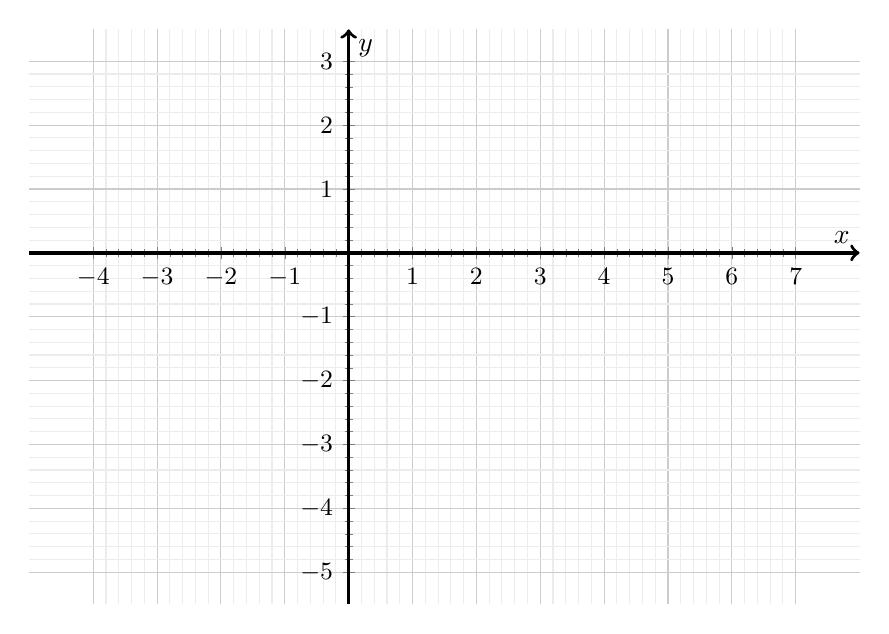
\begin{tikzpicture}
        \begin{axis}[
                xmin=-5, xmax=8,
                ymin=-5.5, ymax=3.5,
                axis lines=middle,
                grid=both,
                minor tick num=4, % ergibt 5 kleine Kästchen pro Einheit
                major grid style={gray!40},
                minor grid style={gray!15},
                axis line style={->, very thick},
                xlabel={$x$},
                ylabel={$y$},
                xtick={-4,-3,...,7},
                ytick={-5,-4,...,3},
                enlargelimits=false,
                grid style={gray!30},
                width=\textwidth,
                axis equal image,
                %height=10cm,
                tick label style={font=\small},
                clip=false
            ]
        \end{axis}
    \end{tikzpicture}
\end{center}
\subsubsection*{Graph einer quadratischen Funktion in quadratisch ergänzter Form (auch Scheitelform genannt)}
\[g:  y=2(x+5)^2+8\]
Man kann direkt ablesen, dass $g$ an $x=-5$ ihren kleinsmöglichen Wert $y=8$ annimmt.

\begin{description}
    \item[Öffnung:] Die Parabel ist nach oben geöffnet.
    \item[Scheitelpunkt:] $\displaystyle S=(-5,8)$
    \item[y-Achsenabschnitt:] $g(0)=58$
    \item[x-Achsenabschnitt:] Der tiefste Wert der Funktion ist positiv, \textbf{g besitzt also keine Nullstellen}
\end{description}
\begin{center}
    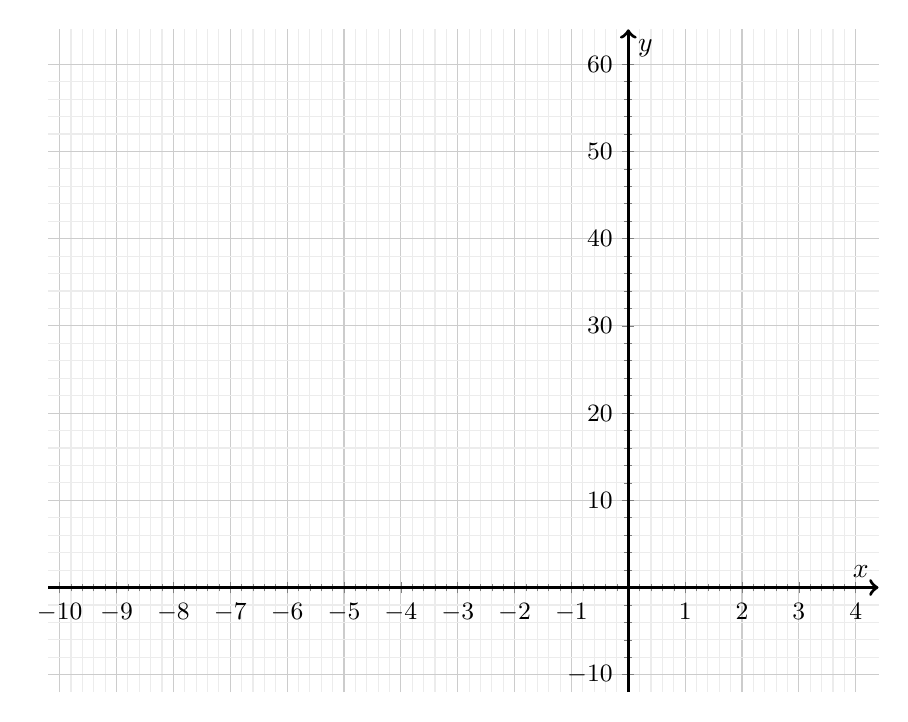
\begin{tikzpicture}
        \begin{axis}[
                xmin=-10.2, xmax=4.4,
                ymin=-12, ymax=64,
                axis lines=middle,
                grid=both,
                minor tick num=4, % ergibt 5 kleine Kästchen pro Einheit
                major grid style={gray!40},
                minor grid style={gray!15},
                axis line style={->, very thick},
                xlabel={$x$},
                ylabel={$y$},
                xtick={-10,-9,...,4},
                ytick={-10,0,...,60},
                enlargelimits=false,
                grid style={gray!30},
                width=\textwidth,
                height=10cm,
                tick label style={font=\small},
                clip=false
            ]
        \end{axis}
    \end{tikzpicture}
\end{center}
\subsubsection{Übungen}
\begin{enumerate}
    \item Wie sieht man an der Funktionsgleichung einer quadratischen Funktion, ob die Parabel nach oben oder nach unten geöffnet ist?
    \item Was hat der Parameter $c$ für einen Einfluss auf die Gestalt des Graphen einer quadratischen Funktion $y=ax^2+bx+c$?
    \item Wahr oder falsch?
          \begin{enumerate}
              \item Alle quadratischen Funktionen sind gerade Funktionen.
              \item Es gibt quadratische Funktionen ohne Nullstellen.
              \item Es gibt keine quadratische Funktion mit genau einer Nullstelle.
              \item Es gibt keine quadratische Funktion mit drei oder mehr Nullstellen.
              \item Da der Graph der Normalparabel mit wachsendem  $x > 0$  immer steiler wird, wird er also ab einer bestimmten Stelle senkrecht sein.
              \item Falls  $a < 0$  ist, ist der Graph der quadratischen Funktion  $x\mapsto ax^2+bx+c$  nach unten geöffnet, ganz unabhängig davon, wie die restlichen Koeffizienten gewählt werden.
              \item Den Graphen der Funktion  $x \mapsto x^2   + 2021$  erhält man, indem man die Normalparabel um 2021 Einheiten in y-Richtung verschiebt.
              \item Der Term $(x+3)^2$ nimmt stets Werte grösser oder gleich 3 an, egal, was man für x einsetzt.
              \item Der Term $4.7\cdot (x-6)^2$ nimmt seinen kleinsten Wert (nämlich 0) einzig dann an, wenn man für x die Zahl 6 einsetzt.
              \item Der Term  $− 7\cdot ( x + 1 )^2+ 5$  nimmt seinen höchsten Wert (nämlich 5) einzig dann an, wenn man für x die Zahl 1 einsetzt.
          \end{enumerate}
    \item Zeichnen Sie den Graphen der Funktion mit der gegebenen Gleichung ohne Wertetabelle in ein Koordinatensystem. Geben Sie die Koordinaten des Scheitels $S$ sowie die Nullstellen an.
          \begin{enumerate}
              \item $y=(x+2)^2$
              \item $y=-\left(x-\dfrac{11}{4}\right)^2-2$
              \item $y=2x^2-4x$
              \item $y=-\dfrac{1}{2}x^2+6x-7$
          \end{enumerate}
    \item Gegeben sind die Graphen A bis H und 12 Funktionsgleichungen. Welche Parabelgleichung gehört zu welchem Graphen?
          \begin{multicols}{3}
              \begin{enumerate}[label=(\arabic*)]
                  \item \(y=x^2-1\)
                  \item \(y=(x+1)^2\)
                  \item \(y=(x-1)^2\)
                  \item \(y=(x+2)^2+1\)
                  \item \(y=(x+2)^2-1\)
                  \item \(y=\frac12(x-1)^2+2\)
                  \item \(y=\left(-\frac12x\right)^2\)
                  \item \(y=-\frac14x^2\)
                  \item \(y=-\frac13x^2-2x\)
                  \item \(y=x^2+6x+5\)
                  \item \(y=x^2-6x+5\)
                  \item \(y=-\frac13x^2+2x\)
              \end{enumerate}
          \end{multicols}
          \begin{center}
              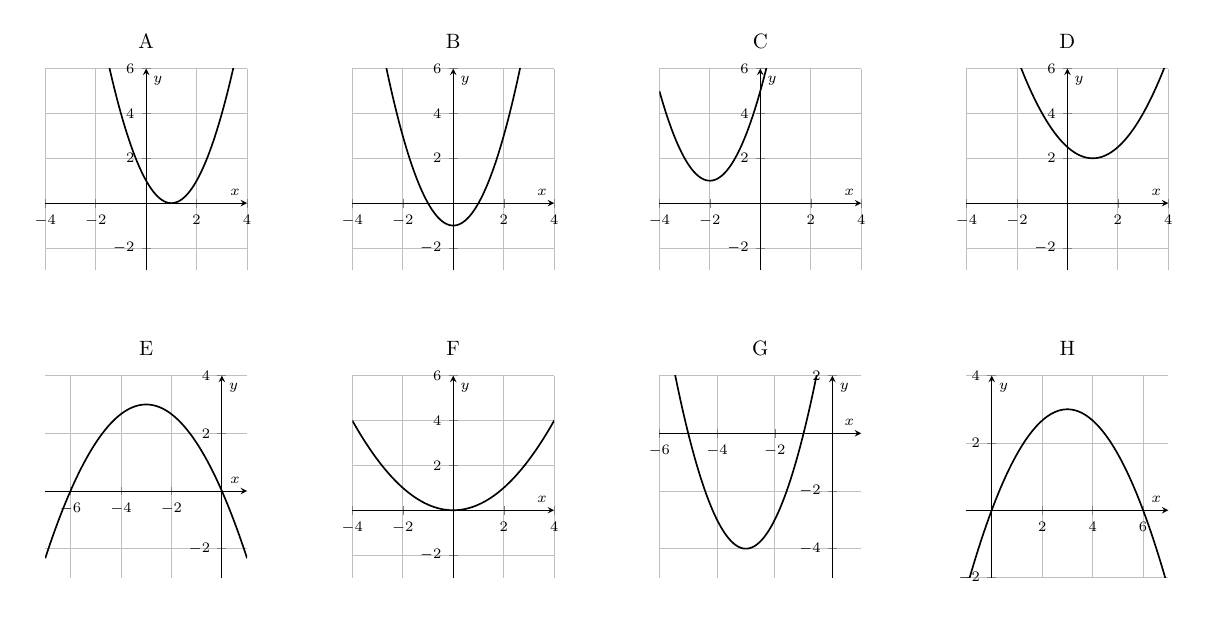
\begin{tikzpicture}[scale=0.75]
                  \pgfplotsset{
                      myaxis/.style={
                              axis lines=middle,
                              xmin=-4, xmax=4,
                              ymin=-3, ymax=6,
                              width=5cm, height=5cm,
                              grid=both,
                              minor tick num=0,
                              xlabel={$x$},
                              ylabel={$y$},
                              tick label style={font=\scriptsize},
                              label style={font=\scriptsize},
                              samples=100,
                              domain=-4:4
                          }
                  }

                  % A
                  \begin{axis}[myaxis, title={A}]
                      \addplot[thick] {(x-1)^2};
                  \end{axis}

                  % B
                  \begin{axis}[myaxis, title={B}, xshift=5.2cm]
                      \addplot[thick] {x^2 - 1};
                  \end{axis}

                  % C
                  \begin{axis}[myaxis, title={C}, xshift=10.4cm]
                      \addplot[thick] {(x+2)^2 + 1};
                  \end{axis}

                  % D
                  \begin{axis}[myaxis, title={D}, xshift=15.6cm]
                      \addplot[thick] {0.5*(x-1)^2 + 2};
                  \end{axis}

                  % E
                  \begin{axis}[myaxis, title={E}, yshift=-5.2cm, xmin=-7, xmax=1, ymin=-3, ymax=4]
                      \addplot[thick, domain=-7:1] {-1/3*x^2 - 2*x};
                  \end{axis}

                  % F
                  \begin{axis}[myaxis, title={F}, xshift=5.2cm, yshift=-5.2cm]
                      \addplot[thick] {0.25*x^2};
                  \end{axis}

                  % G
                  \begin{axis}[myaxis, title={G}, xshift=10.4cm, yshift=-5.2cm, xmin=-6, xmax=1, ymin=-5, ymax=2]
                      \addplot[thick, domain=-6:1] {x^2 + 6*x + 5};
                  \end{axis}

                  % H
                  \begin{axis}[myaxis, title={H}, xshift=15.6cm, yshift=-5.2cm, xmin=-1, xmax=7, ymin=-2, ymax=4]
                      \addplot[thick, domain=-1:7] {-1/3*x^2 + 2*x};
                  \end{axis}

              \end{tikzpicture}
          \end{center}
    \item Wie kann man $x_S$ aus den Nullstellen berechnen, falls der Graph einer quadratischen Funktion zwei Nullstellen $x_1$ und $x_2$ hat? \textit{Tipp: Machen Sie ein Skizze!}
\end{enumerate}
\newpage
\subsubsection*{Lösungen}
\begin{enumerate}
    \item Der Koeffizient $a$ vor $x^2$ gibt die Öffnung an: Ist $a>0$, ist die Parabel nach oben geöffnet, ist $a<0$, ist sie nach unten geöffnet.
    \item Der Parameter $c$ verschiebt den Graphen der quadratischen Funktion in y-Richtung. Je grösser $c$ ist, desto weiter wird der Graph nach oben verschoben, je kleiner $c$ ist, desto weiter wird der Graph nach unten verschoben.
    \item
          \begin{enumerate}
              \item Falsch. Nur wenn $b=0$ ist, ist die Funktion gerade.
              \item Wahr. Zum Beispiel hat die Funktion $f(x)=x^2+1$ keine Nullstellen.
              \item Falsch. Zum Beispiel hat die Funktion $f(x)=x^2$ genau eine Nullstelle, nämlich $x=0$.
              \item Wahr. Denn die Nullstellen einer quadratischen Funktion sind die Lösungen einer quadratischen Gleichung, und eine quadratische Gleichung kann höchstens zwei Lösungen haben.
              \item Falsch. Der Graph der Normalparabel wird zwar immer steiler, aber er wird niemals senkrecht.
              \item Wahr. Denn die Öffnung wird nur durch den Koeffizienten $a$ bestimmt, unabhängig von den anderen Koeffizienten.
              \item Wahr.
              \item Falsch. Der Term $(x+3)^2$ nimmt stets Werte grösser oder gleich $0$ an, nicht grösser oder gleich $3$.
              \item Wahr. Für $x=6$ ist der Term gleich $0$.
              \item Falsch. Der Term nimmt seinen höchsten Wert $5$ an, wenn $x=-1$ ist nicht $x=1$.
          \end{enumerate}
    \item \begin{minipage}[t]{0.8\textwidth}
              \vspace{0pt}

              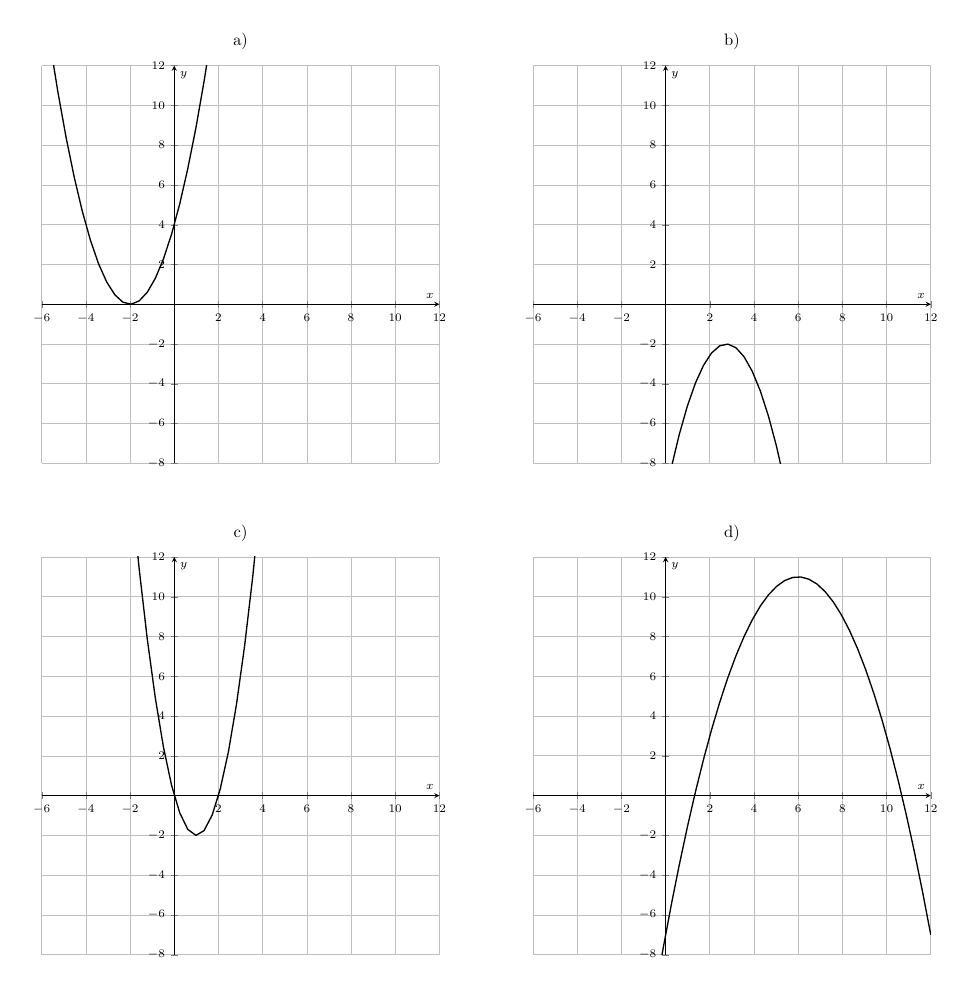
\begin{tikzpicture}[scale=0.6]
                  \pgfplotsset{
                      myaxis/.style={
                              axis lines=middle,
                              xmin=-6, xmax=12,
                              ymin=-8, ymax=12,
                              width=10cm, height=10cm,
                              grid=both,
                              minor tick num=0,
                              xlabel={$x$},
                              ylabel={$y$},
                              tick label style={font=\scriptsize},
                              label style={font=\scriptsize},
                              samples=50,
                              domain=-6:12
                          }
                  }

                  % A
                  \begin{axis}[myaxis, title={a)}]
                      \addplot[thick] {(x+2)^2};
                  \end{axis}

                  % B
                  \begin{axis}[myaxis, title={b)}, xshift=10.4cm]
                      \addplot[thick] {-(x-11/4)^2-2};
                  \end{axis}

                  % C
                  \begin{axis}[myaxis, title={c)}, yshift=-10.4cm]
                      \addplot[thick] {2*x^2-4*x};
                  \end{axis}

                  % D
                  \begin{axis}[myaxis, title={d)}, yshift=-10.4cm, xshift=10.4cm]
                      \addplot[thick] {-0.5*x^2+6*x-7};
                  \end{axis}
              \end{tikzpicture}
          \end{minipage}
    \item \begin{minipage}[t]{\linewidth}
              \vspace{0pt}
              \begin{multicols}{4}
                  \begin{enumerate}[label=(\arabic*)]
                      \item B
                      \item -
                      \item A
                      \item C
                      \item -
                      \item D
                      \item F
                      \item -
                      \item E
                      \item G
                      \item -
                      \item H
                  \end{enumerate}
              \end{multicols}
          \end{minipage}
    \item Aufgrund der Symmetrie des Graphen bezüglich der vertikalen Geraden durch den Scheitelpunkt, liegt der Scheitelpunkt genau in der Mitte zwischen den beiden Nullstellen. Also gilt:
          \[x_S = \frac{x_1 + x_2}{2}\]
\end{enumerate}
\newpage
\subsection{Beispiele Graph $\rightarrow$ Funktionsgleichung}
In diesem Kapitel geht es um die Frage,wie man die Gleichung einer quadratischen Funktion findet, wenn man ausreichende Informationen über den Graphen hat.

Diese Fragestellung kann in der Praxis zum Beispiel dann wichtig sein, wenn man eine Voraussage über die Bahn eines Wurfgegenstandes oder Kometen treffen will.
\subsubsection*{Wenn der Scheitelpunkt bekannt ist}
Gegeben $S=(-2,3),\ P=(5,10)$. Gesucht: Gleichung der quadratischen Funktion, deren Graph den Scheitelpunkt $S$ hat und durch den Punkt $P$ verläuft.
\begin{center}
    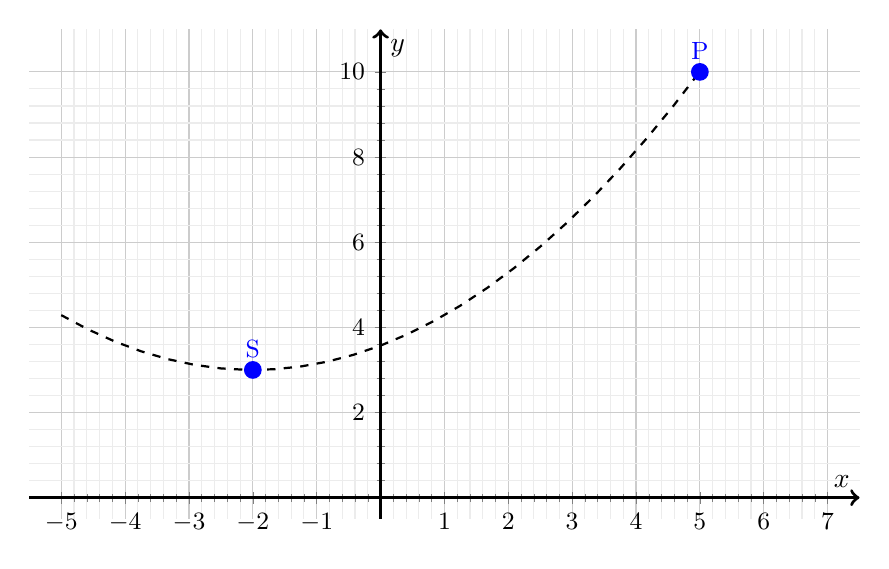
\begin{tikzpicture}
        \begin{axis}[
                xmin=-5.5, xmax=7.5,
                ymin=-0.5, ymax=11,
                axis lines=middle,
                grid=both,
                minor tick num=4, % ergibt 5 kleine Kästchen pro Einheit
                major grid style={gray!40},
                minor grid style={gray!15},
                axis line style={->, very thick},
                xlabel={$x$},
                ylabel={$y$},
                xtick={-5,-4,...,7},
                ytick={0,2,...,10},
                enlargelimits=false,
                grid style={gray!30},
                width=\textwidth,
                axis equal image,
                %height=10cm,
                tick label style={font=\small},
                clip=false,
                x=1.5cm, y=1cm
            ]
            \addplot [thick, dashed] {0.143*(x+2)^2 + 3};
            % Punkt S
            \addplot[only marks, mark=*, mark size=3pt, color=blue] coordinates {(-2,3)};
            \node[blue] at (axis cs:-2,3.5) {\small S};

            % Punkt P
            \addplot[only marks, mark=*, mark size=3pt, color=blue] coordinates {(5,10)};
            \node[blue] at (axis cs:5,10.5) {\small P};
        \end{axis}
    \end{tikzpicture}
\end{center}
\kariert{22}
\newpage
\subsubsection*{Wenn die Nullstellen bekannt sind}
Gegeben sind $x_1=5,x_2=-3$ und $P=(4,1)$. Gesucht ist die Gleichung der Funktion 2. Grades mit den Nullstellen $x_1$ und $x_2$ und einem Graphen, der durch $P$ verläuft.

\begin{center}
    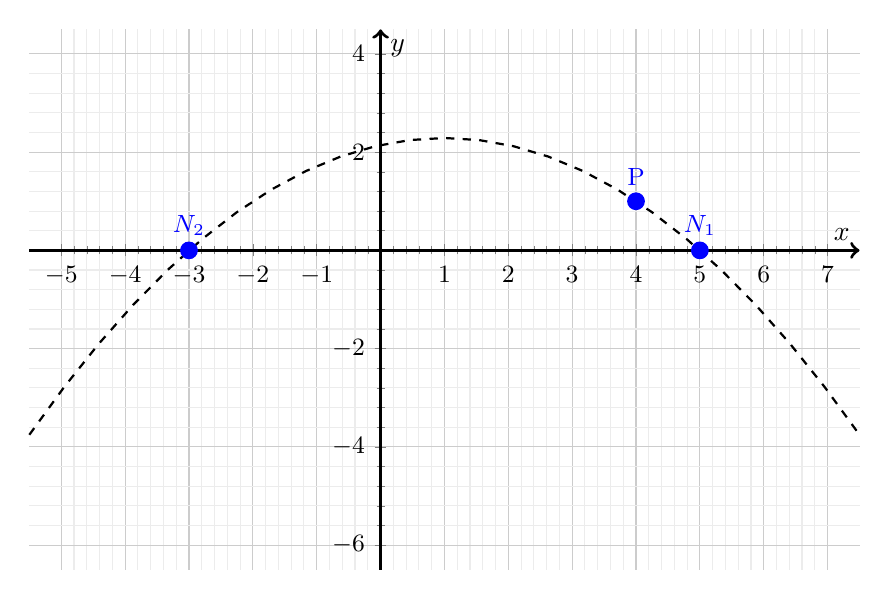
\begin{tikzpicture}
        \begin{axis}[
                xmin=-5.5, xmax=7.5,
                ymin=-6.5, ymax=4.5,
                axis lines=middle,
                grid=both,
                minor tick num=4, % ergibt 5 kleine Kästchen pro Einheit
                major grid style={gray!40},
                minor grid style={gray!15},
                axis line style={->, very thick},
                xlabel={$x$},
                ylabel={$y$},
                xtick={-5,-4,...,7},
                ytick={-6,-4,...,4},
                enlargelimits=false,
                grid style={gray!30},
                width=\textwidth,
                axis equal image,
                %height=10cm,
                tick label style={font=\small},
                clip=false,
                x=1.3cm, y=1cm
            ]
            \addplot [thick, dashed, domain=-5.5:7.5] {-0.143*(x-5)*(x+3)};
            % Punkt N1
            \addplot[only marks, mark=*, mark size=3pt, color=blue] coordinates {(-3,0)};
            \node[blue] at (axis cs:-3,0.5) {\small $N_2$};

            % Punkt N2
            \addplot[only marks, mark=*, mark size=3pt, color=blue] coordinates {(5,0)};
            \node[blue] at (axis cs:5,0.5) {\small $N_1$};

            % Punkt P
            \addplot[only marks, mark=*, mark size=3pt, color=blue] coordinates {(4,1)};
            \node[blue] at (axis cs:4,1.5) {\small P};
        \end{axis}
    \end{tikzpicture}
\end{center}
Eine quadratische Funktion mit den Nullstellen $x_1=5$ und $x_2=-3$ hat eine Gleichung der Form
\[
    f(x)=a(x-5)(x+3)
\]
Der Punkt $P=(4,1)$ liegt genau dann auf dem Graphen von $f$, wenn
\[
    f(4)=1 \iff a(4-5)(4+3)=1 \iff -7a=1 \iff a=-\frac{1}{7}
\]
Die Gleichung der gesuchten Funktion lautet demnach:
\[
    f(x)=-\frac{1}{7} (x-5)(x+3)
\]
und in Normalform:
\[
    f(x)=-\frac{1}{7}x^2+\frac{2}{7}x+\frac{15}{7}
\]
\newpage
\subsubsection*{Wenn drei allgemeine Punkte auf der Parabel bekannt sind}


Gegeben sind die Punkte $A=(2,6),\ B=(4,15)$ und $C=(-4,3)$. Gesucht ist die Gleichung der quadratischen Funktion, deren Graph durch die drei Punkte verläuft.
\begin{center}
    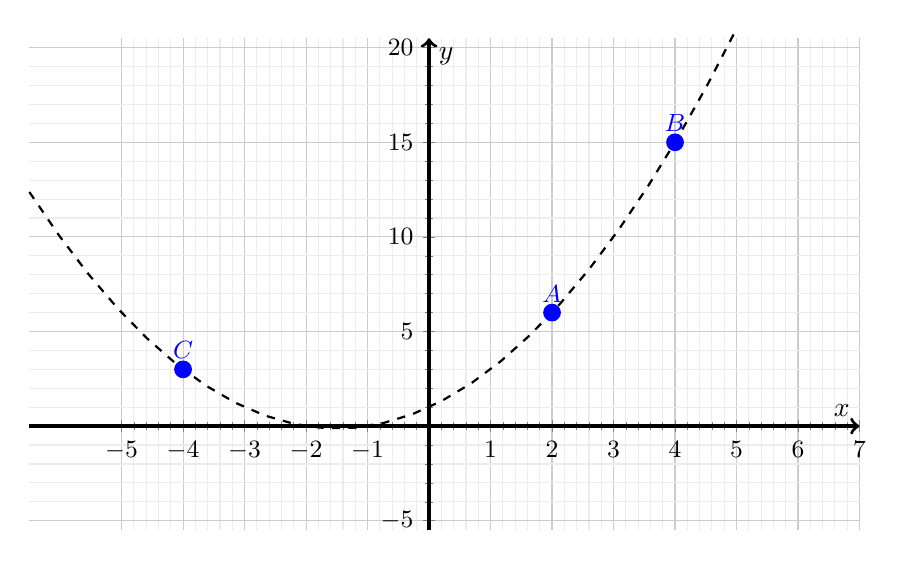
\begin{tikzpicture}
        \begin{axis}[
                xmin=-6.5, xmax=7,
                ymin=-5.5, ymax=20.5,
                axis lines=middle,
                grid=both,
                minor tick num=4, % ergibt 5 kleine Kästchen pro Einheit
                major grid style={gray!40},
                minor grid style={gray!15},
                axis line style={->, very thick},
                xlabel={$x$},
                ylabel={$y$},
                xtick={-5,-4,...,7},
                ytick={-5,0,...,20},
                enlargelimits=false,
                grid style={gray!30},
                width=\textwidth,
                axis equal image,
                %height=10cm,
                tick label style={font=\small},
                clip=false,
                x=1.3cm, y=0.4cm
            ]
            \addplot [thick, dashed, domain=-6.5:5] {0.5*x^2+1.5*x+1};
            % Punkt A
            \addplot[only marks, mark=*, mark size=3pt, color=blue] coordinates {(2,6)};
            \node[blue] at (axis cs:2,7) {\small $A$};

            % Punkt B
            \addplot[only marks, mark=*, mark size=3pt, color=blue] coordinates {(4,15)};
            \node[blue] at (axis cs:4,16) {\small $B$};

            % Punkt C
            \addplot[only marks, mark=*, mark size=3pt, color=blue] coordinates {(-4,3)};
            \node[blue] at (axis cs:-4,4) {\small $C$};
        \end{axis}
    \end{tikzpicture}
\end{center}
\[
    f:  y=ax^2+bx+c
\]
Die drei Punkte $A$, $B$ und $C$ liegen genau dann auf dem Graphen von $f$, wenn
\[
    \begin{cases}
        A\in \text{Graph } f \iff f(2)=6 \iff a\cdot 2^2+b\cdot 2+c=6   \\
        B\in \text{Graph } f \iff f(4)=15 \iff a\cdot 4^2+b\cdot 4+c=15 \\
        C\in \text{Graph } f \iff f(-4)=3 \iff a\cdot (-4)^2+b\cdot (-4)+c=3
    \end{cases}
\]
Das ist ein Gleichungssystem mit drei Gleichungen und drei Unbekannten $a,b,c$! Durch Ausmultiplizieren erhält man
\[
    \begin{cases}
        4a+2b +c = 6 \\
        16a+4b+c=15  \\
        16a-4b+c=3
    \end{cases}
\]
In diesem Fall lassen sich durch geschicktes Kombinieren der Gleichungen, gleichzeitig zwei Unbekannte eliminieren. Dazu bildet man die Differenz der zweiten und dritten Gleichung:
\[
    (2)-(3):  8b=12 \Rightarrow b=\frac{3}{2}
\]
Durch Einsetzen von $b=\frac{3}{2}$ in die Gleichungen (1) und (2) entsteht ein 2x2 System:
\[
    \begin{cases}
        4a+2\cdot \frac{3}{2}+c=6 \\
        16a+4\cdot \frac{3}{2}+c=15
    \end{cases}
    \iff
    \begin{cases}
        4a+c=3 \\
        16a+c=9
    \end{cases}
\]
Die Unbekannte $c$ lässt sich wiederum eliminieren, indem man die Differenz der beiden Gleichugnen bildet:
\[(2)-(1):  12a=6 \Rightarrow a=\frac{1}{2}\]
Schliesslich durch Einsetzen in $(1): 4\cdot \frac{1}{2}+c=3 \iff c=1$.
Die gesuchte Funktion lautet:
\[f(x)=\frac{1}{2}x^2+\frac{3}{2}x+1\]
\newpage
\subsubsection{Übungen}
\begin{enumerate}
    \item Wie lautet die Gleichung \(y=a(x-u)^2+v\) der Parabel mit dem Scheitelpunkt \(S\), die durch den Punkt \(P\) verläuft?
          \begin{multicols}{2}
              \begin{enumerate}[label=\alph*)]
                  \item \(S(2,4),\; P(-1,7)\)
                  \item \(S(2,4),\; P(3,3)\)
                  \item \(S(-2,-3),\; P(0,0)\)
                  \item \(S(2,4),\; P(-6,-12)\)
              \end{enumerate}
          \end{multicols}
    \item Wie lautet die Gleichung \(y=x^2+px+q\) der Normalparabel, die durch die Punkte \(P\) und \(Q\) geht? Berechnen Sie auch die Koordinaten des Scheitels \(S\).
          \begin{multicols}{2}
              \begin{enumerate}[label=\alph*)]
                  \item \(P(2,-7),\; Q(-3,8)\)
                  \item \(P(-1,6),\; Q(4,6)\)
                  \item \(P(7,7),\; Q(-7,-7)\)
                  \item \(P(3,0),\; Q(5,0)\)
              \end{enumerate}
          \end{multicols}
    \item Finde die Gleichung jener Parabel, die durch die Punkte \(P\), \(Q\) und \(R\) geht und bestimme ihren Scheitel \(S\).
          \begin{multicols}{2}
              \begin{enumerate}[label=\alph*)]
                  \item \(P(-4,8),\; Q(0,0),\; R(10,15)\)
                  \item \(P(-3,-3),\; Q(0,3),\; R(3,0)\)
                  \item \(P(1,-1),\; Q(2,4),\; R(4,8)\)
                  \item \(P(-2,10),\; Q(2,10),\; R(3,20)\)
                  \item \(P(1,4),\; Q(4,7),\; R(7,1)\)
                  \item \(P(-3,2),\; Q(-1,-1),\; R(1,-4)\)
              \end{enumerate}
          \end{multicols}
\end{enumerate}
\newpage
\subsubsection{Lösungen}
\begin{enumerate}

    \item
          \begin{enumerate}[label=\alph*)]
              \item \( y = \frac{1}{3}(x - 2)^2 + 4 \)
              \item \( y = -(x - 2)^2 + 4 \)
              \item \( y = \frac{3}{4}(x + 2)^2 - 3 \)
              \item\( y = -\frac{1}{4}(x - 2)^2 + 4 \)
          \end{enumerate}

          \vspace{1em}

    \item
          \begin{enumerate}[label=\alph*)]
              \item \( y = x^2 - 2x - 7,\quad S(1, -8) \)
              \item \( y = x^2 - 3x + 2,\quad S(1.5, -0.25) \)
              \item \( y = x^2 + x - 49,\quad S(-0.5, -49.25) \)
              \item \( y = x^2 - 8x + 15,\quad S(4, -1) \)
          \end{enumerate}

    \item
          \begin{enumerate}[label=\alph*)]
              \item \( y = \frac{1}{4}x^2 - x,\quad S(2, -1) \)
              \item \( y = -\frac{1}{2}x^2 + \frac{1}{2}x + 3,\quad S\left(\frac{1}{2} , \frac{25}{8} \right) \)
              \item \( y = -x^2 + 8x - 8,\quad S(4, 8) \)
              \item  \( y = 2x^2 + 2,\quad S(0, 2)\)
              \item \( y = -\frac{1}{2}x^2 + \frac{7}{2}x + 1,\quad S\left(\frac{7}{2} , \frac{57}{8} \right) \)
              \item  Die drei Punkte liegen auf der Geraden \( g : y = -\frac{3}{2}x - \frac{5}{2} \).
          \end{enumerate}
\end{enumerate}
\newpage

\subsection{Parabel und Geraden}
\subsubsection{Einführungsbeispiel}
Gegeben sind die Parabel $p: y=x^2-2x+4$ und die Gerade $g: y=3x$ (siehe Bild).
\begin{center}
    \begin{tikzpicture}
        \begin{axis}[
                axis lines=middle,
                xlabel={$x$},
                ylabel={$y$},
                xmin=-1, xmax=4,
                ymin=-1, ymax=15,
                samples=200,
                domain=-0.5:5,
                clip=false,
                x=2cm,
                y=0.4cm,
                xtick=\empty,
                ytick=\empty,
            ]
            % Parabel p(x) = x^2 - 2x + 4
            \addplot[thick, blue, domain=-0.5:4.5] {x^2 - 2*x + 4};
            \node[blue] at (axis cs:0.25,4) {$p$};
            % Gerade g(x) = 3x
            \addplot[thick, red] {3*x};
            \node[red] at (axis cs:-0.1,-1) {$g$};
        \end{axis}
    \end{tikzpicture}
\end{center}
Gesucht sind die Koordinaten der Schnittpunkte der beiden Graphen.
\kariert{31}
\newpage
\subsubsection{Versuchen Sie es selbst}
\begin{enumerate}
    \item In welchen Punkten schneidet die Parabel $y=x^2-2x+4$ die Gerade $y=ax$?
          \begin{enumerate}[label=(\alph*), nosep, leftmargin=*, itemjoin={{,\ }}]
              \item $a=-7$
              \item $a=-6$
              \item Was heisst das geometrisch, wenn Parabel und Gerade genau einen Schnittpunkt haben?
          \end{enumerate}
          \kariert{15}
    \item Es gibt zwei Geraden, die durch den Ursprung verlaufen und die Parabel $y=x^2-2x+4$ berühren. Geben Sie deren Gleichungen an.

          Vorgehen: Geraden durch den Ursprung haben eine Gleichung der Form y=ax. Stellen Sie die Gleichung für die Schnittpunkte mit der Parabel auf. Bestimmen Sie dann den Wert von a, sodass die aufgestellte quadratische Gleichung genau eine Lösung hat (Diskriminante = 0)
          \kariert{24}
\end{enumerate}
\subsubsection{Übungen}
Buch Seite 124: 229, 231
\newpage
\subsection{Extremalwertprobleme}
\subsubsection{Einführungsbeispiel 1}
\begin{minipage}{0.5\textwidth}
    Eine rechteckige Weidefläche soll für die Ziege Alma abgezäunt werden. Dabei soll die Weidefläche auf einer Seite durch eine Mauer begrenzt werden und auf den restlichen drei Seiten durch einen 120 m langer Zaun. In welcher Entfernung von der Mauer muss man die Pfosten einschlagen, damit die Weidefläche möglichst gross wird und wie gross wird sie dann?
\end{minipage}
\begin{minipage}{0.5\textwidth}
    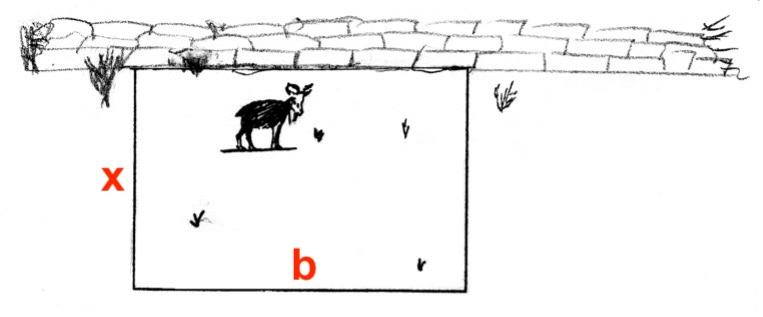
\includegraphics[width=\textwidth]{Quadratische Funktionen/im/Extremalaufgabe1.jpg}
\end{minipage}
\kariert{38}
\subsubsection{Einführungsbeispiel 2}
In der Lös-Bar kostet ein Cappuccino 4 Franken und monatlich werden davon 2000 verkauft. Eine Marktanalyse hat ergeben, dass sich der Absatz $s$ (für sales) in Abhängigkeit des Preises $p$ wie folgt verändert:
\[s=2000-200\cdot (p-4)\]
Das heisst: Pro 1CHF Preiserhöhung verkauft man monatlich 200 Cappuccini weniger– und umgekehrt.

Bei welchem Preis sind die monatlichen Einnahmen am grössten. Wie gross sind dann diese Einnahmen?
\kariert{42}
\newpage
\subsubsection{Übungen}
Buch Seite 127: 253, 255, 259
\newpage
\subsection{Anwendungen}
\subsubsection{Beispiel: Wie weit fliegt der Ball?}
\begin{center}
    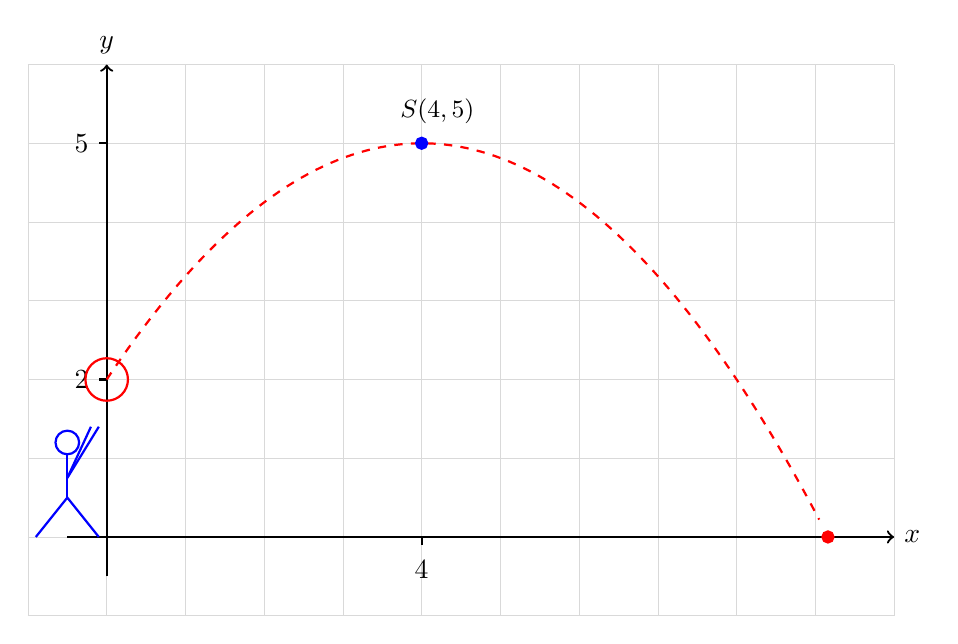
\begin{tikzpicture}[scale=1, thick]
        % Grid
        \draw[step=1cm,gray!30,very thin] (-1,-1) grid (10,6);

        % Achsen
        \draw[->, thick] (-0.5,0) -- (10,0) node[right] {$x$};
        \draw[->, thick] (0,-0.5) -- (0,6) node[above] {$y$};

        % Punkte auf den Achsen
        \foreach \y in {2,5} {
                \draw (0,\y) -- (-0.1,\y) node[left] {\y};
            }
        \draw (4,0) -- (4,-0.1) node[below=2pt] {4};

        % Parabelbahn
        \draw[red, thick, dashed, domain=0:9.05, samples=100]
        plot (\x, {-3/16*\x*\x + 3/2*\x + 2});

        % Startpunkt
        \draw[blue, thick] (-0.9,0) -- (-0.5,0.5) -- (-0.1,0); % Beine
        \draw[blue, thick] (-0.5,0.5) -- (-0.5,1.05); % Körper
        \draw[blue, thick] (-0.5,0.75) -- (-0.1,1.4); % Arm1
        \draw[blue, thick] (-0.5,0.75) -- (-0.2,1.4); % Arm2
        \draw[blue] (-0.5,1.2) circle(0.15); % Kopf
        % Scheitelpunkt
        \filldraw[blue] (4,5) circle(2pt);
        \node at (4.2,5.4) {\small $S(4,5)$};

        % Einschlagpunkt
        \filldraw[red] (9.16,0) circle(2pt);

        % Kreismarkierung um Startpunkt
        \draw[red] (0,2) circle(0.27);

    \end{tikzpicture}
\end{center}
Ein Ball wird vom Punkt $P=(0,2)$ aus geworfen und fliegt auf einer parabelförmigen Bahn. Der höchste Punkt der Bahn ist $S=(4,5)$.

Wie lautet die Gleichung der Flugbahn?
Wie weit fliegt der Ball?
\begin{enumerate}[label=\alph*)]
    \item Wie lautet die Gleichung der Flugbahn?
    \item Wie weit fliegt der Ball?
\end{enumerate}
\kariert{25}
\subsubsection{Übungen}
Seite 125: 236, 237, 241, 243

Gemischte Aufgaben ab Seite 136: alle ungeraden